\documentclass[sigconf]{acmart}

\usepackage{booktabs} % For formal tables

\usepackage{etex}

% Copyright
%\setcopyright{none}
%\setcopyright{acmcopyright}
%\setcopyright{acmlicensed}
\setcopyright{rightsretained}
%\setcopyright{usgov}
%\setcopyright{usgovmixed}
%\setcopyright{cagov}
%\setcopyright{cagovmixed}


% DOI
\acmDOI{10.475/123_4}

% ISBN
\acmISBN{123-4567-24-567/08/06}

%Conference
\acmConference[WOODSTOCK'97]{ACM Woodstock conference}{July 1997}{El
  Paso, Texas USA} 
\acmYear{2017}
\copyrightyear{2017}

\acmPrice{370,000.00}


\begin{document}
\title{Polycommit: Forming Habits Through Gamification}
% \titlenote{Produces the permission block, and
%  copyright information}



\author{Elliot Fiske}
\affiliation{%
	\institution{California Polytechnic State University}
	%  \streetaddress{P.O. Box 1212}
	%\city{Dublin} 
	%\state{Ohio} 
	%\postcode{43017-6221}
}
\email{elliotfiske@gmail.com}

\author{Foaad Khosmood}
\affiliation{%
	\institution{California Polytechnic State University}
}
\email{foaad@calpoly.edu}


\begin{abstract}
\par Learning applications and platforms such as Polylearn are derided for being difficult to use and not engaging. With \textit{Commit,} we demonstrate that through gamification and by learning from user behavior, we can create educational software that improves retention of course content and improves test scores.

\par Using learning techniques such as spaced repitition and variable rewards scheduling, we created a learning platform that is engaging and compelling for users to use. We took favorite features from existing learning platforms such as Duolingo and Memrise, and refined the app's design based on feedback and data from users. Overall, we show that with polish and care shown to the user's motivations, we can create an engaging educational app that students will actually want to use, and enjoy using.

\par We developed \textit{Commit} for use with several Cal Poly classes. We worked directly with teachers to custom-make questions to be used throughout the app. We tested the app in 5 different classes, with around 50 active participats. We found that students who used the application performed 13\% better on tests and recalled 18\% more class knowledge 1 month after completing the course.
\end{abstract}

%
% The code below should be generated by the tool at
% http://dl.acm.org/ccs.cfm
% Please copy and paste the code instead of the example below. 
%
\begin{CCSXML}
<ccs2012>
 <concept>
  <concept_id>10010520.10010553.10010562</concept_id>
  <concept_desc>Computer systems organization~Embedded systems</concept_desc>
  <concept_significance>500</concept_significance>
 </concept>
 <concept>
  <concept_id>10010520.10010575.10010755</concept_id>
  <concept_desc>Computer systems organization~Redundancy</concept_desc>
  <concept_significance>300</concept_significance>
 </concept>
 <concept>
  <concept_id>10010520.10010553.10010554</concept_id>
  <concept_desc>Computer systems organization~Robotics</concept_desc>
  <concept_significance>100</concept_significance>
 </concept>
 <concept>
  <concept_id>10003033.10003083.10003095</concept_id>
  <concept_desc>Networks~Network reliability</concept_desc>
  <concept_significance>100</concept_significance>
 </concept>
</ccs2012>  
\end{CCSXML}

\ccsdesc[500]{Computer systems organization~Embedded systems}
\ccsdesc[300]{Computer systems organization~Redundancy}
\ccsdesc{Computer systems organization~Robotics}
\ccsdesc[100]{Networks~Network reliability}

% We no longer use \terms command
%\terms{Theory}

\keywords{Education, Gamification}

\maketitle



\begin{abstract}
	\par Computer-assisted learning is older than Turing machines, and constantly evolves as technology improves. While some teachers are resistant to using technology in the classroom \cite{BJET:BJET12051}, ``e-learning'' techniques are becoming more common in almost every school, from K-12 to universities \cite{EJED:EJED12020}. As technology becomes more widespread, it becomes crucial to examine the various methodologies of computer-assisted learning and find the techniques that are most effective.

\par This paper explores the effectiveness of one such methodology, spaced repetition. This technique applies to homework assignments available to students online. We include an exploration of several existing apps that use this technique, and introduce our own novel app, \textit{Polycommit.} \textit{Polycommit} was developed for use with several Cal Poly classes and was deployed during the first half of the Spring 2017 quarter. With careful attention to user feedback, we created a tool that motivated students to form better study habits. While our results do not show statistically significant improvement to student grades, this tool gives insight into how modern technology and gamification can be leveraged to create an engaging app that encourages positive study habits.
\end{abstract}


\pagestyle{plain}

\renewcommand{\baselinestretch}{1.66}

\chapter{Introduction}

\section{Learning Technology}

% WHAT SHOULD GO HERE?
% Introduction to spaced repetition
% Survey of learning technologies used
% Gamification explained, stigma, some stuff about Skinner maybe?

\par Learning technology is becoming nearly universally used in classrooms, to the point where some teachers refer to it as "mandatory." \cite{BJET:BJET12051} Yet there is still a "great variation in university lecturers' use of technology," with some teachers not even ready to replace their overhead slides with Powerpoint.

\par We will address the different methodologies teachers use to integrate technology with the classroom, paying special attention to gamification techniques and spaced repetition.

\section{Definitions}

\subsection{Spaced Repetition}

\par In this paper, we introduce \textit{Commit}, a novel web-based application that uses spaced repitition and gamification elements to educational courses. For this thesis, \textit{Commit} was deployed to a variety of classes at California Polytechnic State University to measure its effect on student engagement and learning.

\subsection{Why College Classes?}
\par \textit{Commit} was tested with classes at California Polytechnic State University to facilitate the creation of questions and evaluation of the application. While the app would work with any level of education from K-12 to higher education, using Cal Poly classes allowed us to easily create questions for classes that we had just taken

%\par Gamifying in education has several hurdles. Gamification tends to come with a negative stigma; teachers often feel that gamified services aren't as "serious" as other learning technologies. In addition, existing education gamification solutions have usability issues and are not accessible to students that don't have a background in videogames.

\section{Spaced Repetition}
\par One of the key aspects of Commit is its use of spaced repetition. Spaced repetition is an idea first brought into the mainstream by Pimsleur in the 1960s. Spaced repetition is a learning technique where students reinforce learned knowledge at specific intervals, improving long-term retention and recall ability.

\begin{figure}[h]
	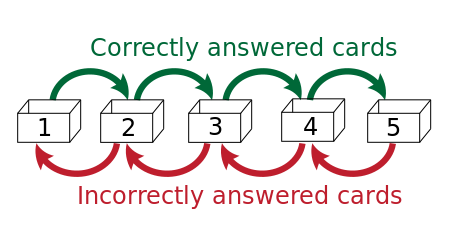
\includegraphics{figures/leitner}
	\caption{The Leitner system. If a student answers a flashcard correctly, it is moved to a higher-numbered box that is reviewed less frequently.}
	\label{fig:leitner}
\end{figure}

\par A simple example of spaced repitition is known as the Leitner system. Flashcards are organized into numbered boxes. (See \textbf{\hyperref[fig:leitner]{Figure \ref*{fig:leitner}}}). Each successive box is reviewed less frequently. That is, a student would review Box 1 twice per day, Box 2 once per day, Box 3 every 2 days, and so on. If a card is answered correctly, it is moved to a box that is reviewed less frequently. However, if the student answers incorreclty, the card is moved to a box that is reviewed more frequently.

\par Thus, tougher cards are reviewed more often, and cards the student knows will be reviewed less often. However, all cards are \textit{eventually} reviewed, and even cards that the student always answers correctly are reviewed in the long term.

\par There is strong evidence that this idea of "spaced repitition" enhances long-term memory and deepens understanding of subject material. \cite{edge2012memreflex}

%[http://www.memorylifter.com/fileadmin/publications/Spacing_Effect_and_Mnemonic_Strategies.pdf]

\section{Spaced Repitition Apps}
\subsection{Duolingo}

\begin{figure}
	%\centering
	\centerline{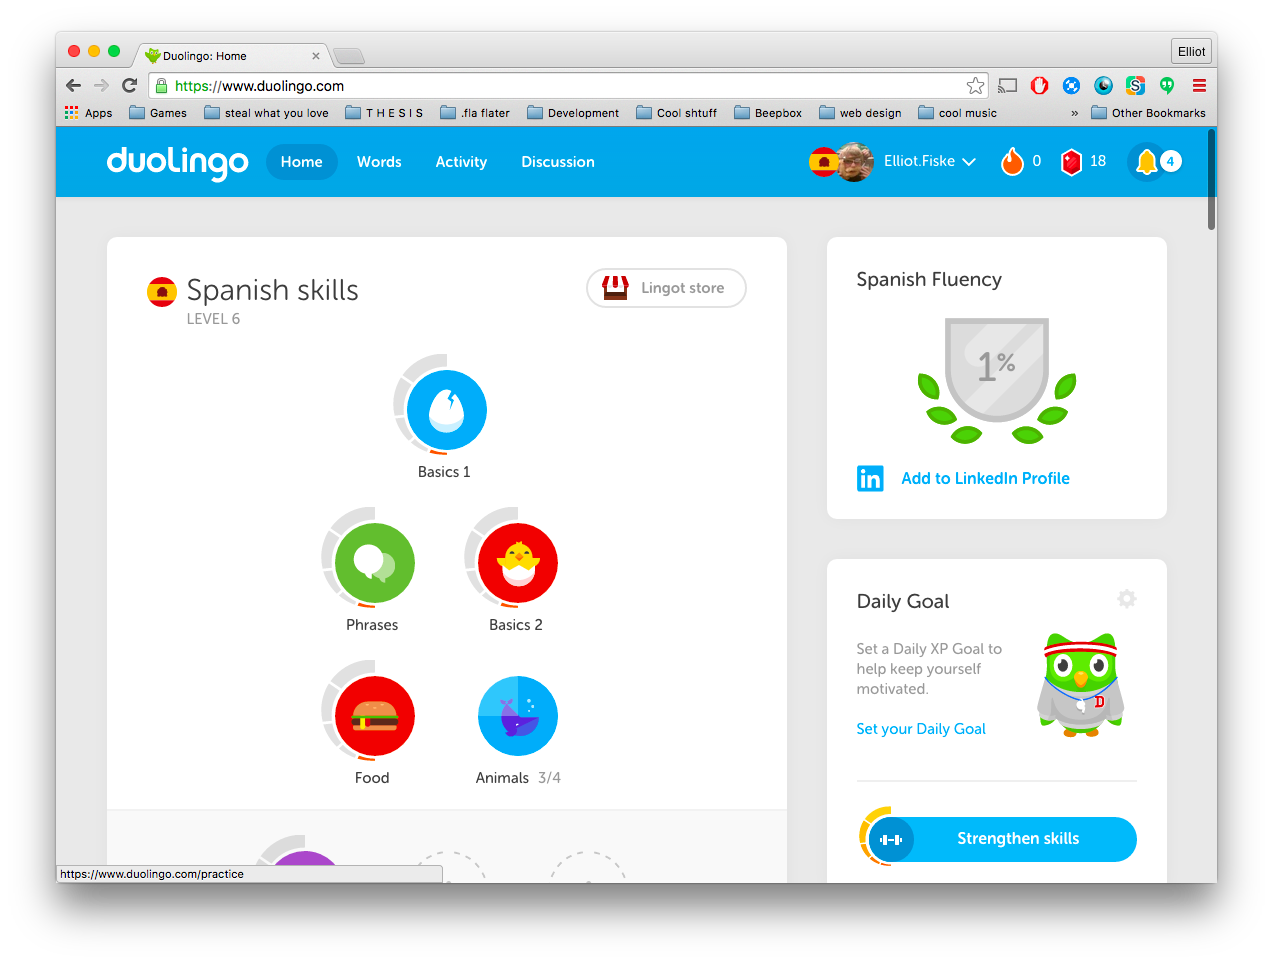
\includegraphics[width=1.2\linewidth]{duolingo}}
	\caption[Duolingo]{The Duolingo interface. Notice the gamification elements and the encouragement to reach a "daily goal."}
	\label{fig:duolingo}
\end{figure}

\par Several recent apps and products make use of spaced repitition to allow user to easily gain long-term recall of languages, class content, or any other information that needs to be learned. One such app is Duolingo (See \textbf{\hyperref[fig:duolingo]{Figure \ref*{fig:duolingo}}}); in Duolingo, users learn a language by repeating small tasks every day. 

\par The app encourages users to spend a small amount of time each day studying useful words and phrases, rather than cramming in a lot of knowledge at once. It encourages this behavior through the use of gamification. Each user earns "experience" in a language, eventually leveling up. Users connect their Facebook accounts and can see their friends' levels and accomplishments, adding a social element to the app.

\subsection{Memrise}

\begin{figure}
	\centering
	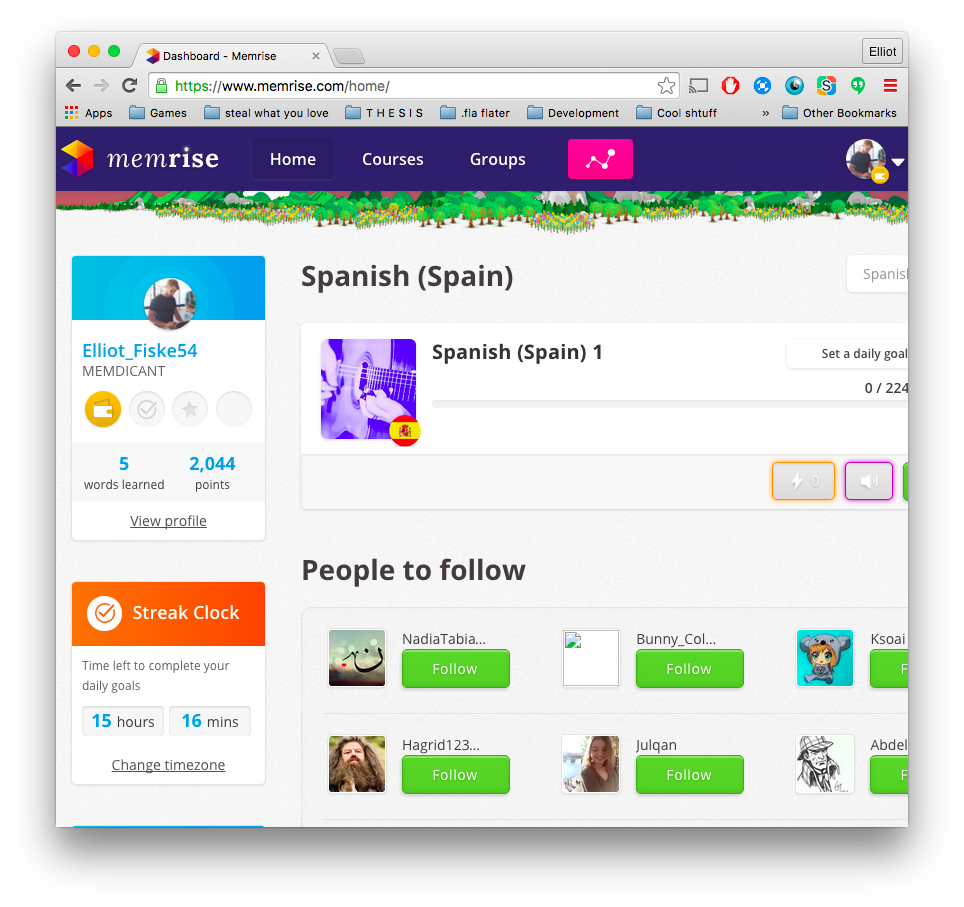
\includegraphics[width=0.7\linewidth]{memrise}
	\caption[Memrise]{Screenshot of the Memrise interface. Note the gamification elements, the social aspect, and the "Streak" clock encouraging consistent use of the app.}
	\label{fig:memrise}
\end{figure}

\par Memrise (See \textbf{\hyperref[fig:memrise]{Figure \ref*{fig:memrise}}})is a web app that has very similar function to \textit{Commit.} Memrise takes a series of flashcard-based questions and answers and automatically creates a "study plan" where the application breaks up flash cards and uses spaced repitition to encode the information in the user's long-term memory. Memrise also uses gamification and social elements, as users earn points for every correct answer and can see their friends' scores.

\par Interesting to note is that users can input any data they choose into Memrise to receive a custom study-guide. This would allow students to easily learn flashcards if they took the time to input them into the app.

\par Both of these applications heavily emphasize language learning, since the process of learning a language can easily be broken down into a series of small words and phrases, and re-emphasized using the process of spaced repitition. However, Commit is scoped specifically to one class, allowing students to easily learn and retain class content without the commitment of adding their own flashcards.

\section{Gamification}
\par The \textit{Commit} app is structured to incentivize students to enjoy using it. The primary incentive for experimental participants was the chance at winning a \$20 Amazon gift card. However, in order to actually obtain this reward the participants would have to engage with the app's systems.

\par One powerful technique used by Commit is the idea of variable rewards scheduling. Variable rewards scheduling is based off of the idea that it's boring to always receive the same reward for performing the same action. It's far more exciting and engaging to not know what reward you'll receive; several studies affirm that variable reward scheduling leads to more willingness to perform a desired target action \cite{dodin2001integrated}.

\par In order to earn entries into the \$20 gift card raffle, participants are required to earn a certain number of \textbf{points.} These points are earned through answering questions. However, far more points are earned if the user returns to the app every day. In addition, "bonus rewards" will be awarded at random intervals to engage users more. The expectation that today may be the "bonus reward" day leads to greater user engagement with the system.

\par In general, users reported that they enjoyed the gamification sections and the potential to earn rewards. Through the study in general, we note that users showed higher rates of engagement and improvements in test scores over the control group that did not use the app.
\chapter{Background}
\section{Early Computing}

\subsection{Pressey and Skinner}
\par The earliest learn

% TODO: fix me
\par Learning applications have been used since the early days of computing. In 1958, BF Skinner \cite{skinner1958teaching} explained how computers could be used to facilitate learning. When Dr. Skinner wrote his paper, computers were already used to test students about subjects that were easy to drill. Dr. Skinner believed that computers would completely revolutionize classrooms. Students would be able to learn at their own pace, with the computer determining the optimal schedule for each student based on how they were performing. Skinner argued that the main advantages of computers as teachers were that students are encouraged "to take an active role in the educational process," 


% NO
and notes that the practice of using automation dates back even to the 1920's with Sidney L. Pressey's automated testing machines. One huge advantage that Pressey noted with automated learning is that students learn at their own pace; one of the toughest challenges teachers face, according to Pressey, is that some students will fall behind while others feel bored because they already understand most of the material being taught. While Pressey's automated teaching methods eventually succumbed to the fact that technology at the time wasn't up to the task of automating education. Instead, Skinner was able to use the technology of his time to more effectively bring computers to the field of education.

% TODO: MAke sure it's clear how this ties into the thesis. Bring up the fact that we're trying to change people's behavior.
\subsection{Behavior and Learning}

% TODO: Define behavior, tie it in to learning, tie it into habits.

\par 

Of course, BF Skinner is famous for his creation of the "Skinner Box," \cite{skinner1963operant} a device that gave simple reinforcement to animals or humans in the lab in order to slowly shape their behavior, through a process known as operant conditioning. When a subject performed well according to the test, they would receive a quick reward, while if they strayed from the purpose of the test, they would not receive a reward. Dr. Skinner argued that "much of what we know [about the learning process] has come from studying the behavior of lower organisms, [and] the results hold surprisingly well for human subjects" \cite{skinner1958teaching}.

\subsection{Variable Ratio Reinforcement Scheduling}
 This method is combined with other interesting motivational techniques such as variable rewards scheduling \cite{ferster1957schedules} \cite{hardy_heyes_1999}, where rewards are not actually doled out on a regular basis exactly according to the behavior of the test subject. Instead, rewards are handed out semi-randomly, varying in quantity and quality, while still mostly rewarding the desired behavior that the researcher is trying to condition. This causes the test subject to become conditioned much faster (See \textbf{\hyperref[fig:variable_ratio]{Figure \ref*{fig:variable_ratio}}}).
 
 \begin{figure}[h]
 	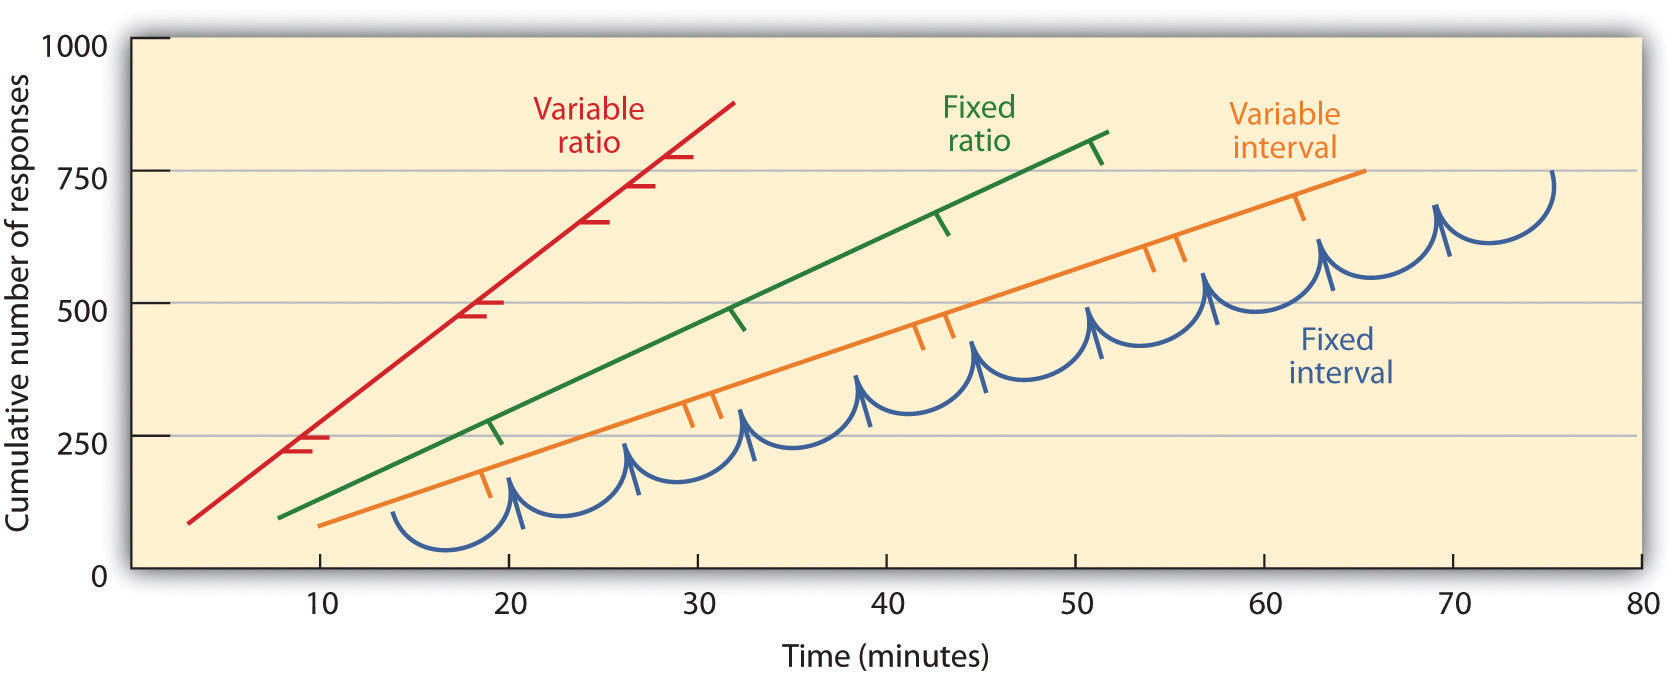
\includegraphics[width=1.0\linewidth]{figures/variable_ratio}
 	\caption{Variable ratio rewards scheduling. Note that as rewards are spaced out randomly, the desired behavior appears much more quickly.}
 	\label{fig:variable_ratio}
 	\cite{hardy_heyes_1999}
 \end{figure}

% TODO: Why is this here? Shouldn't it be in related works
\section{Duolingo}
As mentioned previously in the introduction, Duolingo is an app that already uses several of the processes that we are describing. Duolingo has been shown to be very effective for learning new languages, even perhaps more effective than typical classes. However, the effectiveness of Duolingo is mostly contingent on the motivation of the student. If the student is going to a foreign country soon, Duolingo is the most effective since there is a significant time pressure and pressure to learn the language in order to fit in at whatever country the student is planning to go to \cite{vesselinov2012duolingo}. If, however, the student is simply learning another language for fun, there will be significantly less benefit to them. We must consider this as we develop our educational software; apparently the nature of the student's motivation and their reason for wanting to learn the subject material plays heavily into wheter or not they will be successful in using the app.

\section{Habits}
The study on Duolingo notes how difficult it is to actually get people to use the app. It is extremely hard to change people's habits, taking a lot of time and effort on the user's part to effectively change their behavior. One such strategy around this is to connect one desired "habit" behavior to an existing habit \cite{lally2010habits}. For instance, test subjects in the study by Dr. Lally determined that it was easiest to condition subjects to perform some action by instructing them to perform it right after eating breakfast in the morning. By using the powerful force behind an existing habit, it is possible to "reprogram" your behavior such that a new habit is formed with the new desired behavior.

For instance, if a subject wants to make a habit of cleaning their room, they can make a habit of picking up one piece of clothing after coming home from work for the day. In this way, the habit is driven forward by the regular schedule of coming home at a regular time each day. By associating one behavior with an existing behavior, it is possible to rewire a subject's brain to complete the second behavior far more often.

% TODO Need to read this paper + book in-depth and get a good idea of how habit forming applications go down.
\subsection{New Psychological Theories}
It's interesting to note that the advent of "apps" and habit-forming application has created an essentially new field in psychology \cite{renfree2016don}. In a study, Dr. Renfree argues that the behavior modifications seen in apps like Lift and Memrise actually represent new advances into how habit-forming psychology operates.

% TODO Also expand on this part. The DARK SIDE of gamification, yo
Unfortunately, most of these new effects are actually negative. For instance, Dr. Renfree notes that oftentimes the new habits generated by these apps are "fragile," since they are so dependent on a tight dopamine-based reinforcement loop. As soon as the loop is broken, the brain "loses interest" and the new 
information is deprioritized. This will be an interesting consideration as we develop our application. We want to ensure that the habits and knowledge developed by our app is not simply impermanent, and that it won't be simply "pushed out" by new information.
\chapter{Related Work}

\section{Habit-Forming Apps}
\subsection{Duolingo}

\begin{figure}
	%\centering
	\centerline{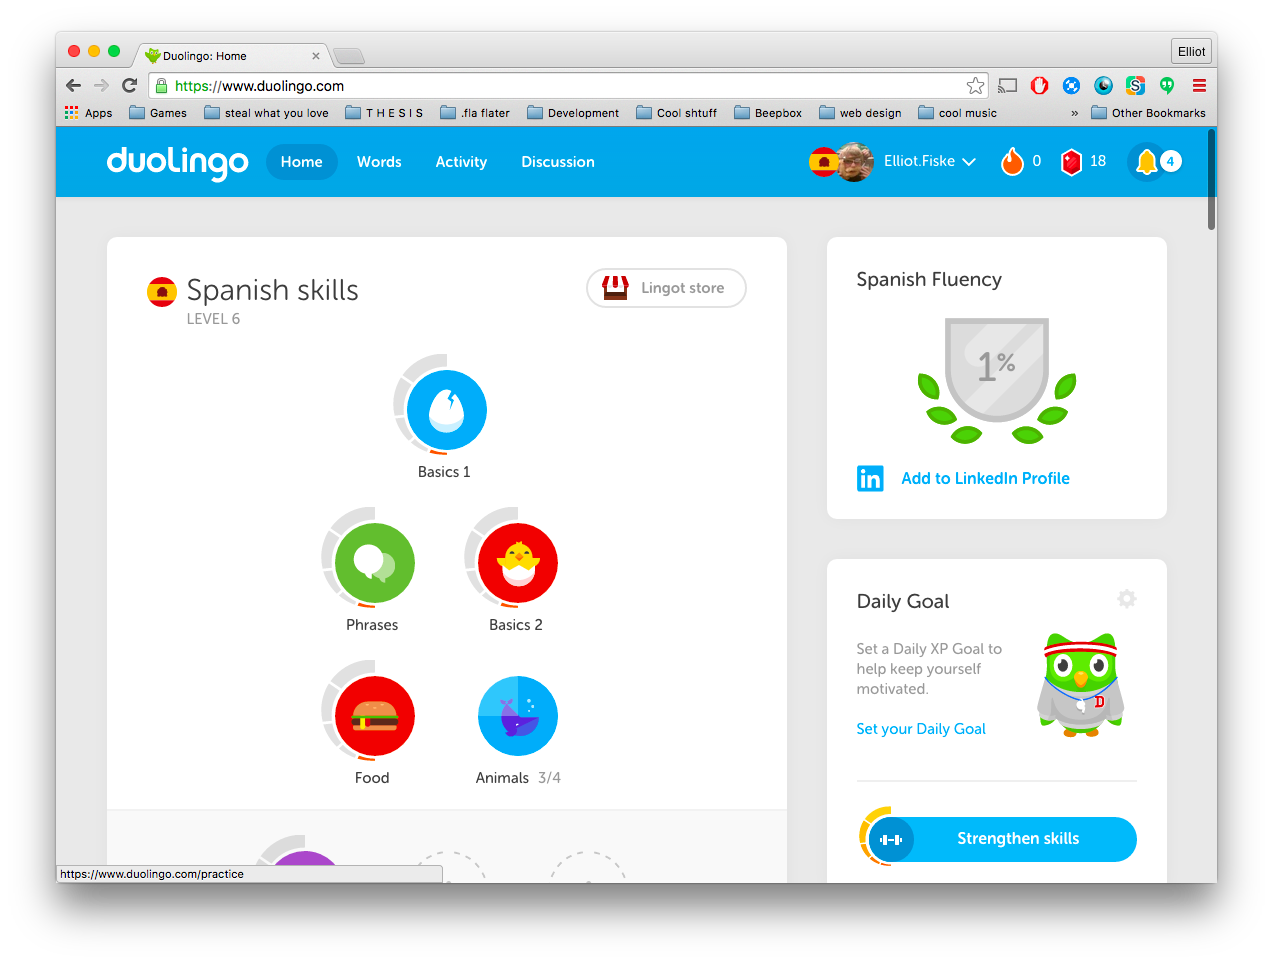
\includegraphics[width=1.2\linewidth]{duolingo}}
	\caption{The Duolingo interface. Notice the gamification elements and the encouragement to reach a ``daily goal.''}
	\label{fig:duolingo}
\end{figure}

\par Several recent apps and products make use of spaced repetition to allow user to easily gain long-term recall of languages, class content, or any other information that needs to be learned. One such app is Duolingo (See \textbf{\hyperref[fig:duolingo]{Figure \ref*{fig:duolingo}}}); in Duolingo, users learn a language by repeating small exercises every day. 

\par The app encourages users to spend a small amount of time each day studying useful words and phrases, rather than cramming in a lot of knowledge at once. It encourages this behavior through the use of gamification. Each user earns ``experience'' in a language, eventually leveling up. Users connect their Facebook accounts and can see their friends' levels and accomplishments, adding a social element to the app. % TODO: Expand on this yo.

\subsection{Memrise}

\begin{figure}
	\centering
	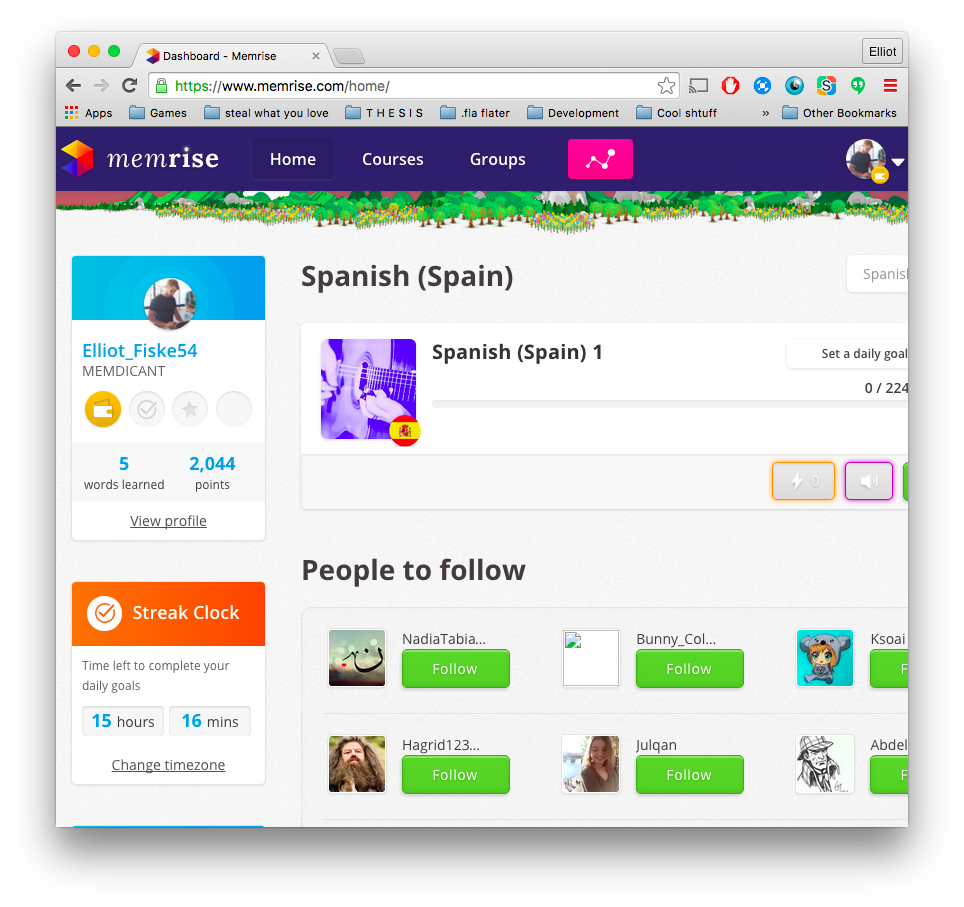
\includegraphics[width=1.0\linewidth]{memrise}
	\caption{Screenshot of the Memrise interface. Note the gamification elements, the social aspect, and the ``Streak'' clock encouraging consistent use of the app.}
	\label{fig:memrise}
\end{figure}

\par Memrise (See \textbf{\hyperref[fig:memrise]{Figure \ref*{fig:memrise}}}) is a web app that has very similar function to \textit{Commit.} Memrise takes a series of flashcard-based questions and answers and automatically creates a ``study plan'' where the application breaks up flash cards and uses spaced repetition to encode the information in the user's long-term memory. Memrise also uses gamification and social elements, as users earn points for every correct answer and can see their friends' scores.

\par Interesting to note is that users can input any data they choose into Memrise to receive a custom study-guide. This would allow students to easily learn flashcards if they took the time to input them into the app.

\par Both of these applications heavily emphasize language learning, since the process of learning a language can easily be broken down into a series of small words and phrases, and re-emphasized using the process of spaced repetition. However, \textit{Polycommit} focuses on one class at a time, allowing students to easily learn and retain class content without the investment of creating their own flashcards.

% end stuff


\subsection{Pocket Points}
\par Pocket Points is an app that attempts to create positive habits for its users through gamification \cite{pocketpoints}. When installed, the app rewards you for keeping your phone locked while in class. It uses GPS to ensure you're on campus, then awards 1 point for every 20 minutes your phone is locked. These points can then be spent to earn discounts and coupons at local businesses. By incentivizing users with discounts and bonuses, Pocket Points attempts to shape its users' behavior.


\begin{figure}
	\centering
	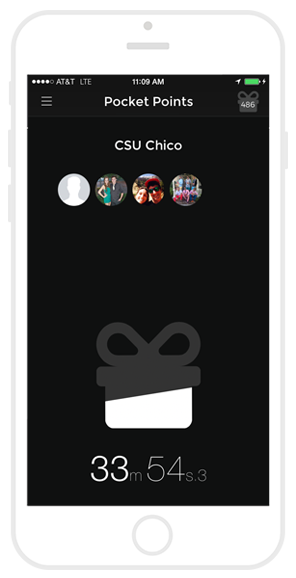
\includegraphics[width=0.7\linewidth]{figures/pocket-points}
	\caption{Screenshot of the Pocket Points interface.}
	\label{fig:pocket-points}
\end{figure}


\subsection{Habit Formation and User Interface}
Previous work has been done to tie habit formation with online user interfaces \cite{johnson2013designing}. In this book, Dr. Jeff Johnson describes how psychology ties into user interface design. He cites that familiar user interfaces lead to less mental stress, encouraging users to come back to your application repeatedly since it seems familiar and less stressful to them. We desire users to consistently use our application every day, so we must keep this in mind. 


\section{Gamification}
Gamification in the classroom has several other examples that can be compared to our application.

\subsection{Classcraft}
Classcraft is an intriguing example of gamification in education (See \textbf{\hyperref[fig:classcraft]{Figure \ref*{fig:classcraft}}}). In Classcraft, students choose a ``role'' and go on the equivalent of a World of Warcraft raid with their fellow classmates. Classcraft is interesting in that it promotes co-operation and a variety of skills, so that students can assist each other where they might not have a certain skill. 

Classcraft takes the typical elements of an RPG and converts them into an experience that supplements a typical classroom experience.

\begin{figure}[h]
	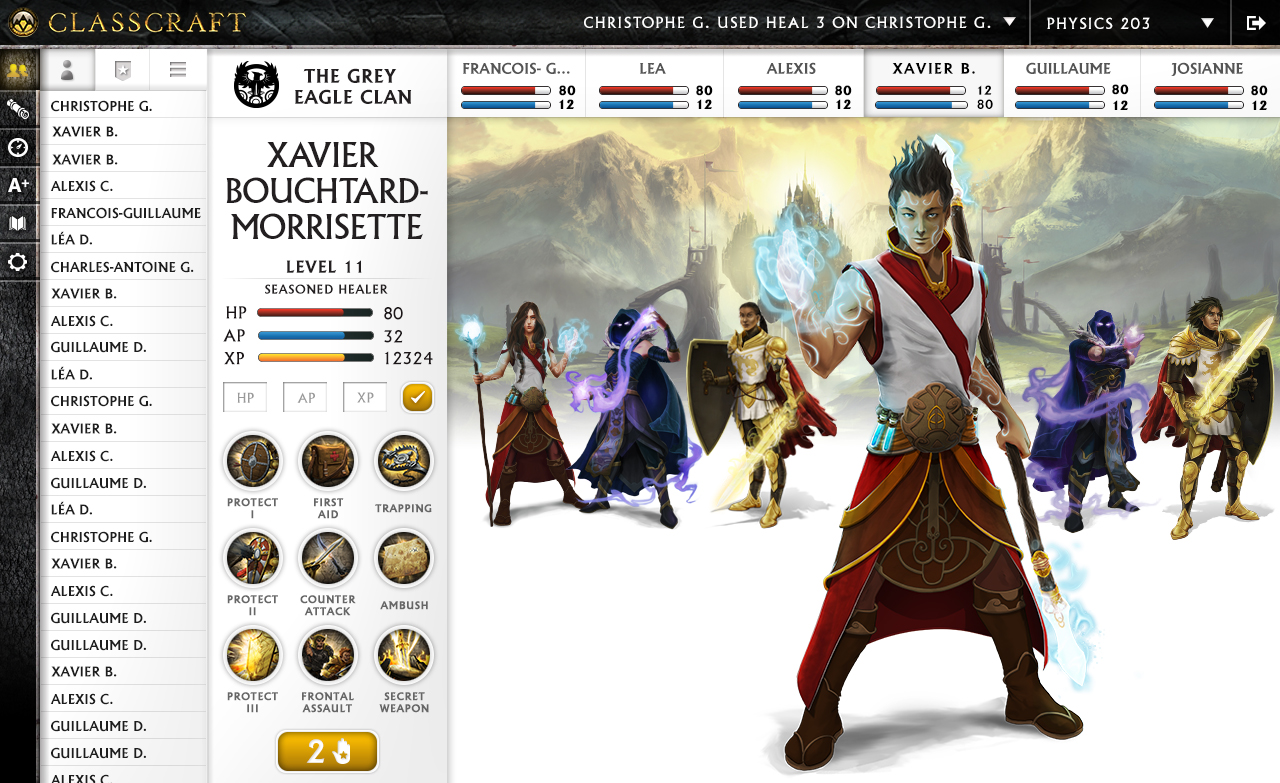
\includegraphics[width=1.0\linewidth]{figures/classcraft}
	\caption{Classcraft user interface. Note the student's health and mana pool, as well as the list of other students in the classroom.}
	\label{fig:classcraft}
\end{figure}

Interesting to note is the emphasis Classcraft puts on integration with existing technologies such as Google Classroom. In order for this application to be widely adopted, it is definitely necessary to have the experience of the teacher go extremely smoothly. Thus, if an application ties directly in with existing technology that the teacher is already familiar with, it will be much more readily adopted by the educational community. It's important to value the teacher's time with this application, so it is necessary to make the UI recognizable, familiar and easy to work with, as well as integrating it with existing tools and perhaps even modeling the user interface after tools that many teachers will already be familiar with.

\subsubsection{Classcraft Study}
A study was done on the effectiveness of Classcraft as well as ``ludicization'' in the classroom in general \cite{sanchez2016classcraft}. Their study ran primarily in France, as this is the home country of the Classcraft company and application. It found that teachers valued the collaborative aspect of Classcraft the most, noting that the app encourages students to work together and support each others' weaknesses rather than compete with one another.

\subsection{Gamification in Other Educational Areas}
So far, we have considered gamification in the classroom mostly in the context of STEM or language fields. While gamification does lend itself towards these subjects, as math problems and science problems can be easily generated by an algorithm, there have also been steps to gamify aspects of classes around liberal arts and the humanities \cite{wagner2017digital}. 

This study by Dr. Wagner approaches a music class the same way Classcraft approaches subjects not focused on the humanity. It highlights the idea of a ``flow'' where a student is fully immersed in the educational process and is fully engaged with the learning process, and notes that it is far easier to attain this ``flow'' state when the student is learning in the context of a video game.
\chapter{Experiment}

\par We carried out an experiment at California Polytechnic State University to test the efficacy of habit-based educational software. We created a web-based application called \textit{Polycommit} that was connected to 4 college classes: \textbf{Introduction to Computer Networks}, \textbf{Introduction to Computer Graphics}, \textbf{Introduction to Computer Networks}, \textbf{Introduction to Operating Systems}, and \textbf{Linear Analysis I}. These classes were selected because they covered subject matter that was easy to convert to online quizzes. For instance, one staple Linear Analysis problem is to find the determinant of a matrix (often a whole number), which is easy to input into an online form. In addition, I had taken these classes in recent quarters and was familiar with the course content.

\par We presented \textit{Polycommit} to each of the courses in the first 2 weeks of class. Students voluntarily signed up through a website hosted at https://polycommit.com/.

\section{UI Overview}

\subsection{Home Scren}
\par Upon logging in, students click ``Enroll'' for the classes they wish to participate in. Upon enrolling, the classes are listed under the ``Enrolled Classes'' section (\textbf{\hyperref[fig:polycommit1]{Figure \ref*{fig:polycommit1}}}). This page also lists the two main ``scores'' that students earn by answering questions: \textbf{Commitment} and \textbf{Points}.

\par Commitment is a numerical value that represents how many \textit{unique} days a student has answered a question on the website. Students could earn up to 1\% extra credit on their final grade in the class by getting 15 Commitment.

\par Points are earned by answering questions. More points are awarded for correct answers, and bonus points are awarded based on the user's current Commitment. All participants in the experiment were placed in a raffle for \$20 Amazon gift cards. Additional entries into the raffle were awarded by earning more points.

\begin{figure*}[h]
	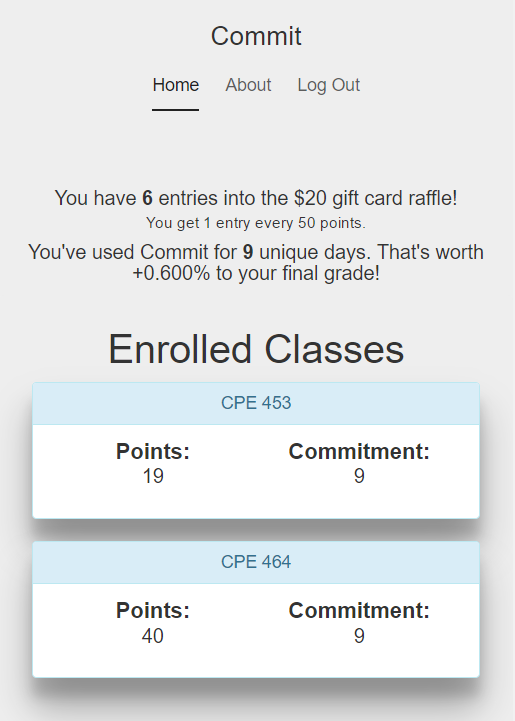
\includegraphics{figures/polycommit-screen}
	\caption{The ``Home'' screen for \textit{Polycommit}. Students can see their current progress and can click on a course to answer challenges.}
	\label{fig:polycommit1}
\end{figure*}

\subsection{Course Screen}
\par Each course page has a list of challenges (\textbf{\hyperref[fig:polycommit2]{Figure \ref*{fig:polycommit2}}}) that are open to the student. Challenges are grouped by the week in which they are opened. If a student has completed all the challenges in a week, the week is displayed with a green check mark and does not expand. If there are open challenges in a week, the week is displayed in yellow with an ``alert'' icon, indicating that the student has an available challenge. This UI imparts a sense of urgency to the user, since they could potentially lose opportunities to earn Commitment by not answering a question in a 24-hour period. Each challenge also lists the date it was opened, and the number of points awarded if the challenge is already completed.

\par Finally, the Course page lists the student's points and Commitment for the course, along with a tooltip that explains what ``Commitment'' is. The Commitment and Point values are repeated from the Home page since they are central to the experience of the app, and it is inherently satisfying to watch your points and Commitment rise as you complete challenges.

\begin{figure*}
	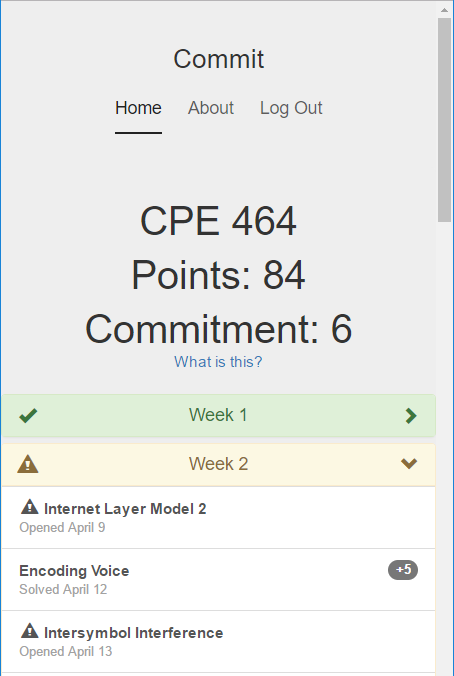
\includegraphics{figures/polycommit-challenges}
	\caption{The ``Course'' screen for Polycommit. Students can see their current Points and Commitment and can see a list of challenges organized by date.}
	\label{fig:polycommit2}
\end{figure*}

\subsection{Challenge Screen}
\par The challenge screen is where students see the content of a challenge and input their answers. A challenge can either be Multiple Choice, Short Answer, or Numerical. An example of a simple Multiple Choice challenge is at \textbf{\hyperref[fig:polycommit3]{Figure \ref*{fig:polycommit3}}}.

\par At the bottom of the Challenge screen is a link to submit feedback about a question. Through this link, students are brought to a Google form where they can provide feedback about a particular question. The feedback form is viewable at \textbf{\hyperref[fig:polycommit4]{Figure \ref*{fig:polycommit4}}}.

\par Once the challenge is closed, students can see a list of their previous attempts along with the correct answer to the problem. Certain problems have their answers hidden; for instance, all Linear Analysis problems don't show their answers because many challenges on \textit{Polycommit} are directly from the assigned homework. Hiding the correct answer prevents students from quickly inputting a wrong answer to see the homework solutions. Additionally, if a question has received feedback as being confusing, an ``Explanation'' field provides detailed context about the answer the problem and potential pitfalls (See  \textbf{\hyperref[fig:polycommit5]{Figure \ref*{fig:polycommit5}}}).

\begin{figure*}
	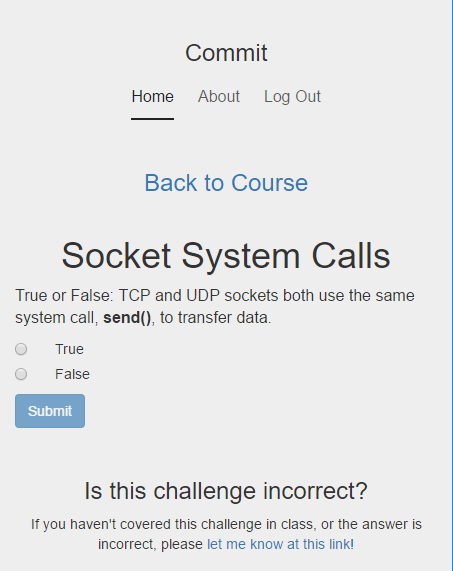
\includegraphics{figures/pc-question}
	\caption{The ``Challenge'' screen for Polycommit. Students see the content of the challenge and can enter their answers. At the bottom is a link where students can give feedback on a challenge.}
	\label{fig:polycommit3}
\end{figure*}


\begin{figure*}
	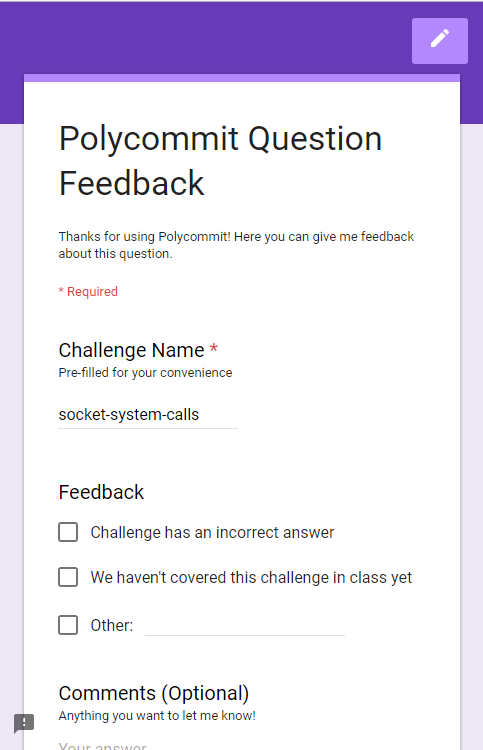
\includegraphics{figures/pc-feedback}
	\caption{The Feedback form for questions. The id for the question is automatically filled in. The student can optionally enter their email address (off-screen) if they want to be contacted when the challenge is fixed.}
	\label{fig:polycommit4}
\end{figure*}

\begin{figure*}
	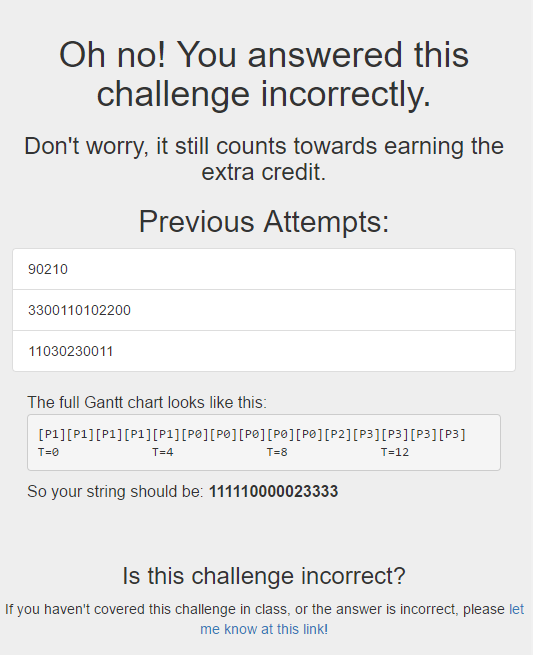
\includegraphics{figures/pc-incorrect}
	\caption{The view of a challenge once it has been answered incorrectly. The main message assures the user that it still counts for Commitment. A full explanation of the problem is under the list of the user's attempts.}
	\label{fig:polycommit5}
\end{figure*}

\subsection{Toasts}
\par \textit{Polycommit} uses ``toasts'' to convey temporary, state-based information to the user. For instance, when the user answers a question, they get immediate feedback in the form of a pop-up toast. Positive information, such as a correct answer, is styled with a green background and a check mark. Negative information, such as an incorrect answer or a server error, is bright red with an alert symbol that commands the user's attention. Examples of each are at \textbf{\hyperref[fig:polycommit6]{Figure \ref*{fig:polycommit6}}}.


\begin{figure*}
	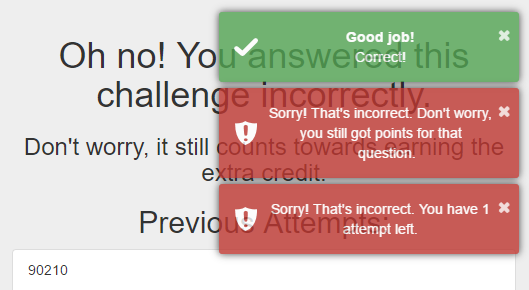
\includegraphics{figures/pc-toast}
	\caption{Three examples of ``toast'' notifications. These provide useful state-based information, such as whether a challenge was answered correctly. They also can provide feedback if an error occurred, such as a challenge not submitting due to poor network connectivity.}
	\label{fig:polycommit6}
\end{figure*}

\section{Technology Used}
\par All the code for \textit{Polycommit} is available here:
\hyperref[https://github.com/elliotfiske/commitment]{https://github.com/elliotfiske/commitment}

\par \textit{Polycommit} has its origins in a Summer 2016 section of Dynamic Web Development (CPE 437), taught by Dr. Clint Staley. The base code and overall code architecture remain, as well as some of the platforms used. The app runs on a M*EAN stack. It uses Node.js as a backend, with Express as a routing service and MySQL as a database. In addition, Sequelize is used to easily interface with the database from Javascript. Angular.js is used as a frontend framework, supplemented by Bootstrap for reactive layout.

\par Node.js and Javascript lends itself well to quick, iterative development. As a dynamically typed language with first-class and anonymous functions, it is easy to quickly make sweeping changes based on user feedback. However, since Javascript is an interpreted language, potential errors that a compiler could have caught may make it through to the live site. Because of this, it was extremely important to regularly run the backend code through comprehensive unit tests.

\subsection{Test-First Methodology}
\par All of the backend server code is thoroughly covered by various test cases. I used the service \textit{Postman} to maintain a suite of tests that ensured all the data involved in \textit{Polycommit} was both available and secure. \textit{Postman} allows developers to run a series of web requests against a server, and verify that the correct response or error code is returned (See  \textbf{\hyperref[fig:polycommit5]{Figure \ref*{fig:postman}}}). For instance, one test suite logs in as a student and attempts to complete a challenge, create a class, and query the information of another student. Only the first request should complete successfully; the student's unprivileged account should not be able to create classes or see other students' data.

\par Writing test cases for new server functionality \textit{before} beginning development allowed me to see edge cases before they arose, and allowed for the satisfaction of seeing the tests pass as I completed each feature. In addition, it protected the privacy of students' answers and scores.



\section{User Feedback}
\par At the bottom of every page is a link encouraging users to send feedback to my email address (See \textbf{\hyperref[fig:feedbacklink]{Figure \ref*{fig:feedbacklink}}}). Throughout the experiment, I received a large amount of excellent feedback that helped me refine the app's usability.

\subsection{Early Testing}
\par Before the main experiment in Spring 2017, we ran a small dry run of the app to get a general feel for usability issues. The app was announced in CPE 464 in week 6, directly after the midterm. The main difference from the current iteration is the onboarding process. Instead of registering and logging in through the Cal Poly portal, students registered using an email address and had to click a link that was emailed to them to complete registration.

\par We discovered that this onboarding process had an extremely high drop-off rate. Of the 10 people that visited the posted link, only 4 entered their email, and only 2 successfully completed registration. As such, it became a huge priority to reduce the number of steps a user had to complete to begin using the app. Other studies could learn from this process and implement a one-click login process that ensures maximum user participation.

\subsection{Ongoing Feedback}
\par Throughout the experiment, I received feedback from 16 different users consisting of bug reports and feature requests. A full list of the feedback I received is available in <Appendix A>

%Throughout the duration of the experiment, I received a large amount of excellent feedback about the usability of \textit{Polycommit}. At the bottom of each page is a link
%%TODO
%TODO: Finish section on how I used user feedback to improve the app. Include emails from Polycommit folder.

\chapter{Validation}

\par The experiment was carried out over the first half of the Spring 2017 quarter at Cal Poly. 130 students signed up across 4 classes. By the end of the experiment, just over 3200 answers had been submitted to the application.

\section{Data Gathering}

\subsection{Midterm Scores}
\par In order to gauge the effectiveness of \textit{Polycommit}, we collected scores on quizzes and exams and aggregated the data to be analyzed. For \textbf{Introduction to Operating Systems}, data collection was extremely simple as all the quizzes and midterms were administered through an online exam. This allowed us to easily obtain data on how students performed on specific midterm questions that aligned with questions asked in \textit{Polycommit}.

\par However, the other classes were not as simple. The other classes administered paper midterms, and we did not have access to the papers as they were being graded. As such, we administered a secondary survey to all the students in the class asking them to input their midterm scores for various questions.

\subsection{Final Survey}
\par After the experiment was concluded, all participants were sent a link to a survey where they could give feedback about their overall experience using \textit{Polycommit}. As an incentive, any participant who filled out the survey received +3 Commitment and +50 points (equal to an additional entry in the gift card raffle). A total of 70 participants filled out the post-experiment survey.

\subsection{Limitations}
\par Certain tradeoffs were necessary in order to run this experiment.
\subsubsection{No Control Group} 
\par Most importantly, there is no true control group for this experiment. We decided that it would be more advantageous to offer the application to all students in each section of the classes. This simplified the onboarding process, as we could present the application to all members of the class at once, and allow anyone to sign up. It also prevented potential issues where students might perceive it as unfair that certain students were give access to a study resource and others were not. In addition, this allowed more students to participate in the experiment, giving us access to more data and more user feedback.

\par As such, it's important to note that the students who participated in the study \textbf{self-selected} to become part of the experiment. Students who \textbf{did not} use the app can't be considered a control group, because they are not a random selection from the whole population. Allowing students to self-select may have introduced confounding variables. For example, perhaps students who are confident in their study techniques would choose to not participate, making the average midterm scores higher for non-participants.

\subsubsection{Self-Reporting Midterm Scores}
\par As noted above, students were asked to input their midterm scores in an online form. We have no way of determining if this data was accurately entered; students may feel tempted to enter a higher score than they actually received. Note that we \textit{do} have access to the overall midterm scores, so the issue only arises when analyzing individual questions on the exams. Data that has been affected by this issue is clearly marked in the upcoming sections.

\section{Overall Results}
\subsection{Cramming vs. Commitment}
\par First, consider the relationship between a student's overall score on the midterm and their Commitment (\textbf{\hyperref[fig:comm_vs_score]{Figure \ref*{fig:comm_vs_score}}}). 
 
 \begin{figure}[ht]
 	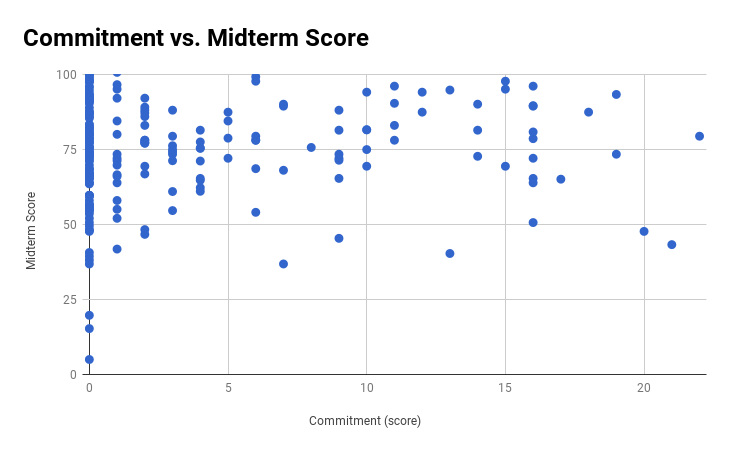
\includegraphics[width=1.0\linewidth]{figures/commitment-data1}
 	\caption{Graph of Commitment versus the student's percentage score for all classes.}
 	\label{fig:comm_vs_score}
 \end{figure}

\par Note that we are showing the midterm percentage score, since the midterms in different classes have different total score values.
\par There is no clear correlation between a user's Commitment value and the score they got on the midterm. Thus, this data does not support the hypothesis that using spaced repetition to study for an exam improves the user's score.

\par  Next, we can compare the total number of questions answered by each user with their midterm score (\textbf{\hyperref[fig:cramming]{Figure \ref*{fig:cramming}}}). If students received a benefit from the Commitment system, we might expect to see \textit{less} of a correlation between total questions answered and midterm score. This is because if a user has a high number of questions answered but a low Commitment, this indicates they answered the questions all at once, in a ``cram'' session. According to our hypothesis, this would not help improve their long-term understanding of the course.

\begin{figure}[ht]
	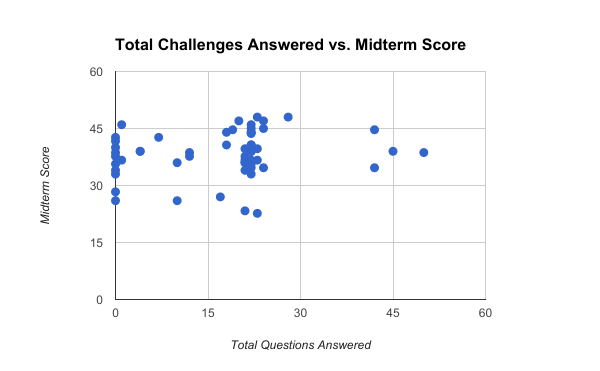
\includegraphics[width=1.0\linewidth]{figures/cramming-data}
	\caption{Graph of Total Questions Answered vs. the student's score on the midterm.}
	\label{fig:cramming}
\end{figure}
 
 \par Next, consider the mean of all midterm scores between students that didn't answer \textit{any} questions vs. the ones that did. For all classes except CPE 471, students that didn't answer any questions in the app scored slightly higher on average than the students that didn't. The discrepancy in CPE 471 is most likely due to the smaller number of students that signed up for \textit{Polycommit}.
 
 \par Note that we define ``Active Users'' as any user with over 5 Commitment. 
  
  \begin{table}
 \begin{tabular}[h]{ r c c c}
  & \textbf{Non-users} & \textbf{All Users} & \textbf{Active Users} \\
  \hline
  \textbf{All Classes} & & & \\
  Midterm Average & 72.93 & 76.12 & 76.88 \\
  Population Size & 119 & 103 & 87 \\
  \hline
  \textbf{CPE 453} & & & \\
 Midterm Average & 74.38 & 77.56 & 77.40 \\
 Population Size & 14 & 46 & 42 \\
 \hline
 \textbf{CPE 464} & & & \\
 Midterm Average & 68.90 & 73.85 & 76.08 \\
 Population Size & 47 & 42 & 34 \\
 \hline
 \textbf{CPE 471} & & & \\
 Midterm Average & 87.38 & 82.39 & 83.83 \\
 Population Size & 34 & 7 & 4 \\
 \hline
 \textbf{MATH 244} & & & \\
 Midterm Average & 74.43 & 85.87 & 85.87 \\
 Population Size & 26 & 11 & 10 \\
 
\end{tabular}
\caption{Average midterm scores for different samples of the population. Note that an ``Active User'' is a user with more than 5 Commitment.}
\end{table}

\subsection{Individual Questions}
Certain questions on the midterm matched closely with the content of the questions that were repeated on \textit{Polycommit}. We can analyze midterm results to see if the students that drilled related problems in \textit{Polycommit} performed better on the related questions during the midterm.

\subsubsection{Introduction to Operating Systems}
One question that was shared between the midterm and \textit{Polycommit} was a question about the 4 conditions for deadlock. The question on the midterm asked students to choose the correct 4 conditions from a series of dropdowns, while the question on \textit{Polycommit} asked students to choose the \textit{incorrect} condition from the list. The 4 conditions for deadlock are:

\begin{enumerate}
	\item \textbf{Mutual exclusion}: At least one resource can only be
	held by one process at a time; this can result in other
	processes waiting for that resources
	\item \textbf{Hold and wait}: A process must be holding at least one
	resource while waiting for other resources (held by other
	processes)
	\item \textbf{No preemption}: Resources can only be released
	voluntarily by a process; Resources cannot be revoked
	\item \textbf{Circular wait}: A set of n waiting process $ {P_0, ..., P_n} $
	such that $ P_i $ is waiting for resources held by $ P_{(i+1)\%n} $
\end{enumerate}

\par The content of the question in \textit{Polycommit} and the question in the midterm are very similar. We can see if individuals who answered the Deadlock question correctly in \textit{Polycommit} had a higher score, on average, than the individuals who did not.

\begin{figure}[th!]
	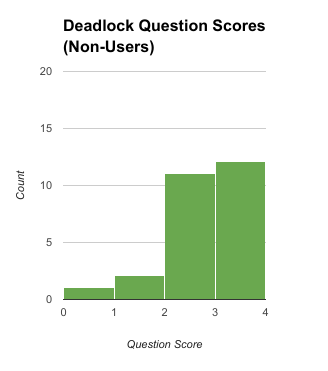
\includegraphics[width=0.5\linewidth]{figures/deadlock-nonusers}
	\caption{Count of scores for students that did \textit{not} make an attempt on the Deadlock question in \textit{Polycommit}.}
	\label{fig:deadlock-no}
\end{figure}

\begin{figure}[h!b]
	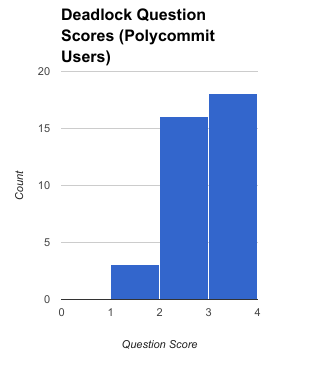
\includegraphics[width=0.5\linewidth]{figures/deadlock-users}
	\caption{Count of scores for students that \textit{did} make an attempt on the Deadlock question in \textit{Polycommit}.}
	\label{fig:deadlock-yes}
\end{figure}

\par The mean score for \textbf{non-users} is 3.30, and the mean score for \textbf{users} is 3.31. Thus, using \textit{Polycommit} had a negligible effect on the average score of the participants. However, note that 23/26 \textbf{non-users} received a score greater than 3, while 34/37 \textbf{users} received a score greater than 3. This could reflect the fact that \textit{Polycommit} only referenced 3 out of the 4 conditions for deadlock, as the 4th condition in the problem was a false plant. Although all 4 conditions are listed in the ``explanation'' field for the problem, by default if a student answers the question correctly they are brought back to the course page. Thus, students who participated in \textit{Polycommit} were only drilled on 3 out of the 4 conditions for deadlock, which would explain the overall performance on the midterm.

\par Next, we will examine problems related to scheduling. Scheduling, in Operating Systems, is the process by which a multithreaded CPU decides which processes get to run at a certain time. Since scheduling problems are easy to generate and automatically grade, several such problems were included in \textit{Polycommit}. Below, we graph the amount of scheduling problems users answered in \textit{Polycommit} versus the score they got on the scheduling section of the midterm (See \textbf{\hyperref[fig:scheduling]{Figure \ref*{fig:scheduling}}}).

% TODO: also include graph where people got the polycommit question incorrect

\begin{figure}[h!b]
	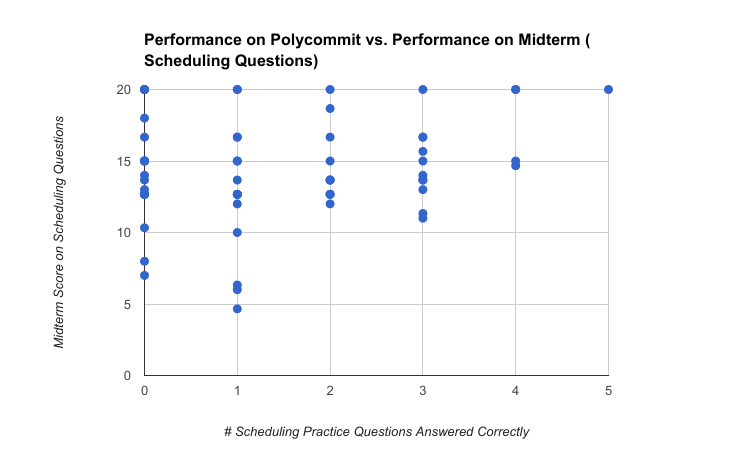
\includegraphics[width=1.0\linewidth]{figures/scheduling}
	\caption{Scatter plot where the X axis is the amount of scheduling problems the user answered on \textit{Polycommit}, and the Y axis is the total score they received on the 4 scheduling questions of the midterm.}
	\label{fig:scheduling}
\end{figure}

\par As you can see, there is a clear correlation between consistently practicing scheduling questions and performing well on the exam. While many students did get full credit on the scheduling portion of the exam, the students who answered all 5 scheduling questions on Polycommit all scored perfectly on that section of the exam.


\subsubsection{Introduction to Computer Graphics}

\par Questions about \textbf{vector math}, \textbf{transformation matrices}, and \textbf{barycentric coordinates} were practiced in \textit{Polycommit}, and were subsequently tested on the midterm for Computer Graphics. Below is a table displaying the midterm performance of students who answered questions about each question on \textit{Polycommit}.

\begin{table}
	\begin{tabular}[h!]{ r c c }
		& \textbf{Did practice} & \textbf{Did not practice} \\
		\hline
		\textbf{Vector Math} & & \\
		Score & 98\% & 100\%  \\
		
		\hline
		\textbf{Transformation Matrices} & &  \\
		Score  & 92.1\% & 86.3\% \\
		
		\hline
		\textbf{Barycentric Coordinates} & &  \\
		Score  & 100\% & 97.7\% \\
		
	\end{tabular}
\caption{IMPORTANT: These midterm scores were self-reported, so their accuracy depends on the honesty of the reporting student.}
\end{table}

\subsubsection{Introduction to Computer Networks}

\par Questions about \textbf{IP Addressing}, \textbf{CRC Checksums} and \textbf{sliding window protocol} were practiced in \textit{Polycommit}, and were subsequently tested on the midterm for Computer Networks. Below is a table displaying the midterm performance of students who answered questions about each question on \textit{Polycommit}.

\begin{table}
	\begin{tabular}[h!]{ r c c }
		& \textbf{Did practice} & \textbf{Did not practice} \\
		\hline
		\textbf{IP Addressing} & & \\
		Score & 80\% & 77.4\%  \\
		
		\hline
		\textbf{CRC Checksums} & &  \\
		Score  & 100\% & 86.3\% \\
		
		\hline
		\textbf{Sliding Window Protcol} & &  \\
		Score  & 90\% & 76.9\% \\
		
	\end{tabular}
\caption{IMPORTANT: These midterm scores were self-reported, so their accuracy depends on the honesty of the reporting student.}
\end{table}

\section {User Feedback}

\par At the end of the experiment, we contacted all of the participants with a final survey that asked them questions about their usage of the app. It also included two free-response questions that asked users to offer suggestions about how the app could be improved.

\subsection{Rating Summary}

\par The full survey is viewable in \textbf{\hyperref[fig:survey1]{Figure \ref*{fig:survey1}}}. Users responded to several statements about the app using a standard Likert scale ranging from Strongly Disagree to Strongly Agree. A summary of the user responses is available at \textbf{\hyperref[fig:likert]{Figure \ref*{fig:likert}}}. Notably, a majority of users responded quite positively to the app.


\begin{figure}[h]
	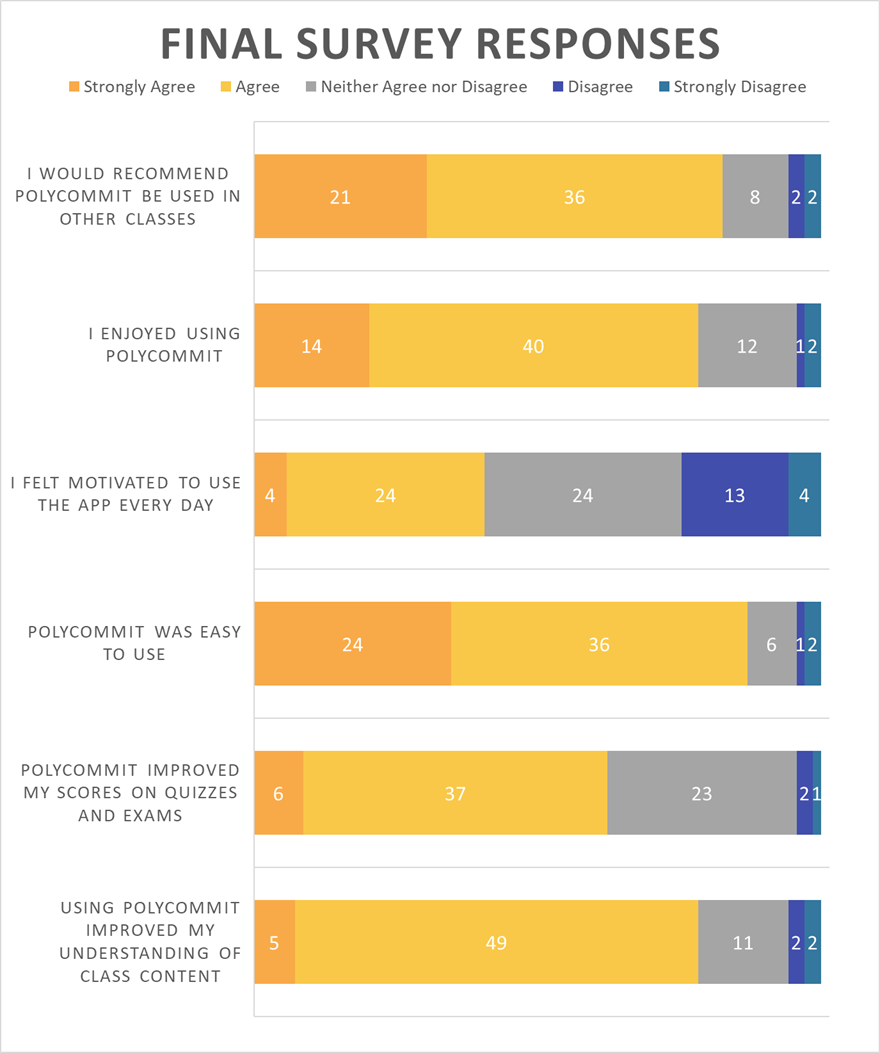
\includegraphics[width=1.0\linewidth]{figures/likert}
	\caption{Survey responses from users of Polycommit.}
	\label{fig:likert}
\end{figure}

\subsection{User Self-Evaluation vs. Actual Scores}

\par One interesting result comes by grouping midterm scores by the user's response to ``\textit{Polycommit} improved my scores on quizzes and exams'' (See \textbf{\hyperref[fig:overconfidence]{Figure \ref*{fig:overconfidence}}}). Students who reported that \textit{Polycommit} did \textit{not} improve their scores scored substantially higher than students who did. One explanation for this is that students who were already confident about their studying habits or had prior knowledge of Operating Systems did not feel that \textit{Polycommit} had an impact on their grades, which are already high overall.

\begin{figure}[h]
	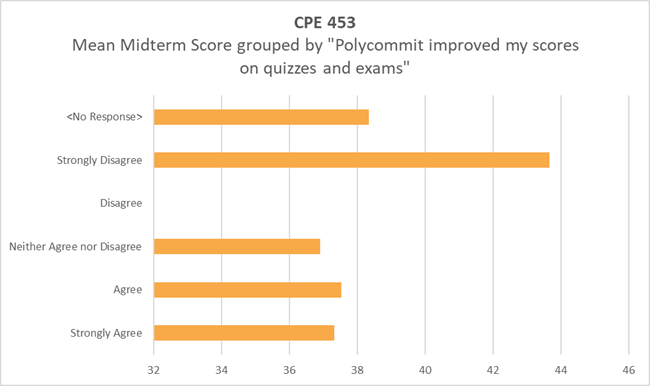
\includegraphics[width=1.0\linewidth]{figures/improved-vs-score}
	\caption{Mean midterm score grouped by response to final survey question ``\textit{Polycommit} improved my scores on quizzes and exams.''}
	\label{fig:overconfidence}
\end{figure}


\subsection{Free Response Summary}
\par Before viewing the results, we predicted some categories that user responses might fall into. These categories are:

\begin{enumerate}
	\item Problems or confusions with the user interface
	\item Questions were not correct or were confusing
	\item Questions did not represent test material
	\item App needed more gamification, excitement, or incentive to use
	\item Other
\end{enumerate}

\par The total number of responses that fell under each category are:

\vspace{1.0cm}

\begin{tabular}{ r c }
	\textbf{Category} & \textbf{\# Responses} \\
	Problems or confusions with the user interface & 26 \\
	Questions were not correct or were confusing  & 9 \\
	Questions did not represent test material  & 5 \\
	App needed more gamification, excitement, or incentive to use  & 1 \\
	Other  & 29 \\
\end{tabular}

\vspace{2.0cm}

\par The full list of responses is available below. Note that answers \textit{are} shown when a question is closed, so feedback asking for answers to be displayed is filed under ``UI Issues'' since the problem is essentially that the app failed to present the information in a way that users could find it.

\input{chapters/UserFeedbackList}



 
\chapter{Conclusion and Future Work}

\par Overall, we have shown little statistical correlation between the use of \textit{Polycommit} and improvements to student grades. However, given the overall positive user feedback received about the app, it may be worthwhile to move forward with the idea of improving student understanding through habit formation and gamification.

\section{Potential Improvements}

% TODO: include a bit in here about "smart questions" that target users' weak spots

\par There are several improvements we could make to the experiment to draw a more definite conclusion about the effect of habit-forming gamification on student performance.

\subsection{Experiment Scope}

\par For the purposes of this thesis, we took a "breadth-first" approach to gathering data. That is, we released the app to a variety of classes (most were advanced Computer Science courses, but each covered completely separate topics) and allowed any students to participate in the experiment. This allowed us to get feedback and data from a variety of different perspectives.

\par However, after refining the experience based on the feedback from the "breadth-first" approach, the next step would be to take a "depth-first" approach to the experiment. That is, we would deploy the app in a more focused manner. We would choose a particular class, such as a introductory Calculus class, and deploy the app to every available section. This would give us more consistent data to work with, as we could compare the performance of different sections of the same class.

\subsection{Control Group}
\par A further improvement to the experiment would be implementing a control group. There are two main ways we could accomplish this. 

\par One method would be to only offer the app to certain sections of a class, while still collecting the scores on quizzes, exams and homework from the non-using sections. This approach has the advantage of being easy to implement, but has the disadvantage of introducing confounding variables to the experiment. The population of students who choose one section over another is not randomly sampled; for instance, students with better studying habits might take a class in an earlier section, causing the average grade on quizzes and exams to be higher in certain sections.

\par Another method would be to only offer the app to a randomly selected sample of students in the class. This has the advantage of being more scientifically sound, as a random sample on a large population would rule out other factors that might affect student performance. However, it would complicate the onboarding process, as we would be unable to present the app to the entire class and allow anyone with a Cal Poly account to sign up. One method would be to have the app be part of a mandatory graded assignment, and send a link to each of the participating students that allows them to sign up. This would hopefully ensure that all the students that were selected to participate would actually engage with the app.

\subsection{Experiment Duration}

\par This experiment took place over the first 5 weeks of Spring Quarter 2017. To gain a more complete understanding of how students respond to the app and how habits are formed over time, it would be advantageous to run further experiments over longer periods of time. Data from different quarters could be compared, adjusting different factors in the experiment to determine how users best respond to gamification. 

\par In addition, several users requested that questions continue past week 5 so they could have a study tool for the final. Future experiments could run for the duration of the whole quarter, allowing us to collect data from all the assignments throughout the quarter, including the final.

\subsection{User Feedback}

\subsubsection{Notifications}

\par As noted in \textbf{\hyperref[feedback-table]{Table \ref*{feedback-table}}}, users requested several additional features and improvements to the UI. One of the most requested features was the ability to receive notifications each day reminding the user to answer a question and thus earn Commitment. I had considered adding this to the app, but received some feedback during the dry run in Winter 2017 that email notifications would be annoying rather than useful. Thus, I chose to focus on other features rather than adding an element that might discourage certain students from using the app. For future experiments, an opt-in email notification system with a easy-to-use "Unsubscribe" option would likely increase user engagement while not annoying users that don't wish to be notified.

\subsubsection{Showing Answers}

\par A number of users requested in the final survey that answers, or answer hints, be shown after completing a question. Originally, the app did not have that feature, but I added it partway into the experiment because several users contacted me about it. The number of students that requested this feature, although it already existed, indicates that the UI does not make it clear that the feature is available. Currently, if students get a question wrong and exceed the maximum number of attempts, the app stays on the page with the closed challenge, and the answer is shown at the bottom of the screen. There could be some other indication that the answer is visible, perhaps on the course page itself.

\par Similarly, to address some user confusion I added an \textit{Explanation} field where I 
\section{Conclusion and Future Work}

\par After we have collected the data from the remaining classes, we can get a more in-depth understanding of how using \textit{Polycommit} affected student understanding of the course material and test scores.

\nocite{*}
% \bibliography{bibliography}

\bibliographystyle{ACM-Reference-Format}
\bibliography{sigproc} 

\end{document}
